
\documentclass{bredelebeamer}

\usepackage{kotex}
\usepackage{amsmath}
\usepackage{minted}
\usepackage{threeparttable}
\usepackage{booktabs}

\DeclareMathOperator*{\minimize}{minimize}
\DeclareMathOperator*{\argmax}{arg\,max}
\DeclareMathOperator*{\argmin}{arg\,min} 
\setminted{fontsize=\footnotesize,baselinestretch=1}
\usemintedstyle{borland}

\def\code#1{\texttt{#1}}

\title[Compiler Project]{컴파일러 프로젝트 발표}

\subtitle{}

\author{김규래, 박건}

\institute[Sogang University]
{
  서강대학교\\
}


\date{June 13 2019}
\subject{Design and Development of Compiler for C- Language}

\fontsize{11pt}{7.2}

%%%%%%%%%%%%%%%%%%%%%%%%%%%%%%%%%%%%%%%%%%%%%%%%%%%%%%%%%%%%%%%%%%%%%
\begin{document}

\begin{frame}
  \titlepage\
\end{frame}

\begin{frame}{발표에서 다룰 내용}
  \tableofcontents %[hideallsubsections]
  % You might wish to add the option [pausesections]
\end{frame}

\section{프로젝트 3 결과}
\subsection{Symbol Table 구현방법}
\begin{frame}{Symbol Table 구현방법}
	\begin{figure}
		\includegraphics[scale=0.3]{images/symtab.png}
	\end{figure}
\end{frame}

\begin{frame}{Symbol Table 구현방법}
	\begin{block}{Linked List of Hash Tables}
		\begin{itemize}
			\item Linked List의 각 노드가 해당 Scope의 Hash Table
			\item Scope에 들어갈 때 \code{st\_enter\_scope()} 함수로 Linked List에 노드 추가
			\item Scope가 종료될 때 \code{st\_exit\_scope()} 함수로 Linked List에서 노드 제거
			\item Semantic Analysis가 끝난 후 Symbol Table의 내용을 각 Scope별로 출력해야 하기 때문에 완전히 제거하지 않고, 따로 저장해 놓음. (\code{next} 필드)
		\end{itemize}
	\end{block}
\end{frame}

\begin{frame}[fragile]{Symbol Table 주요 코드}
	\begin{minted}
	[frame=lines,
	framesep=2mm,
	baselinestretch=0.7]{c}
/* The record in the bucket lists for
* each variable, including name, 
* assigned memory location, and
* the list of line numbers in which
* it appears in the source code
*/
typedef struct BucketListRec {
	const char* name;
	Record record;
	struct BucketListRec* next;
} * BucketList;

/* The local scope symbol table  */
typedef struct LocalSymbolTableRec {
	BucketList hashTable[SIZE];
	struct LocalSymbolTableRec* parent;
	struct LocalSymbolTableRec* next;
} * LocalSymbolTable;
	\end{minted}
\end{frame}

\begin{frame}[fragile]{Symbol Table 주요 코드}
	\begin{minted}
	[frame=lines,
	framesep=2mm,
	baselinestretch=0.7]{c}
void st_enter_scope(SymTable state)
{
    LocalSymbolTable table 
         = malloc(sizeof(struct LocalSymbolTableRec));
    for (int i = 0; i < SIZE; ++i) {
        table->hashTable[i] = NULL;
    }
    table->parent                 = state->currentScope;
    table->next                   = NULL;
    state->currentScope           = table;
    state->lastConstructed->next  = table;
    state->lastConstructed        = table;
}

void st_exit_scope(SymTable state)
{
    state->currentScope = state->currentScope->parent;
}
	\end{minted}
\end{frame}

\subsection{Semantic Analysis 구현방법}
\begin{frame}{Semantic Analysis 구현방법}
	\begin{itemize}
		\item 처음에는 복잡성을 줄이기 위해 Single Pass로 구현
		\item 그러나 나중에 수업시간에 배웠던 대로 Two Pass로 구현을 바꿈.
		\item 그랬더니 실행시간이 줄어듦.
	\end{itemize}
	
	\begin{figure}
		\centering
		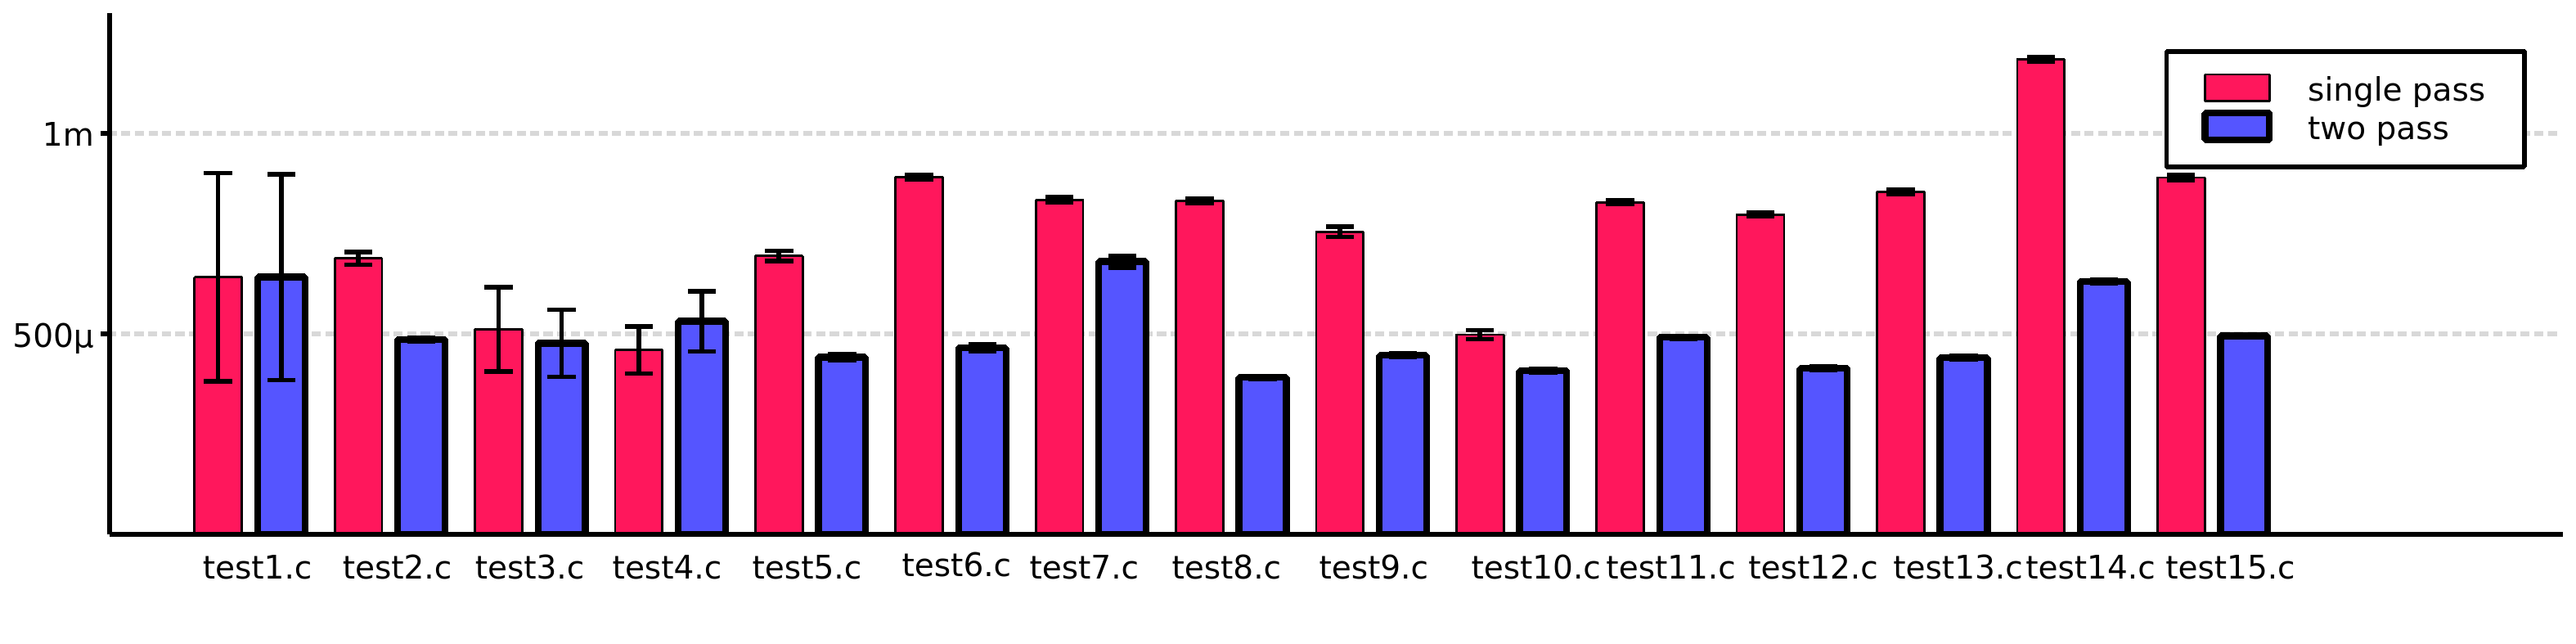
\includegraphics[scale=0.29]{figure/performance.png}
	\end{figure}
\end{frame}

\begin{frame}{Single Pass Runtime Analysis}
	\begin{figure}
		\centering
		\includegraphics[scale=0.5]{figure/onepass_semantic.png}
	\end{figure}
\end{frame}

\begin{frame}{Two Pass Runtime Analysis}
	\begin{figure}
		\centering
		\includegraphics[scale=0.3]{figure/twopass_trace.png}
	\end{figure}
\end{frame}

\begin{frame}{Two Pass Runtime Analysis}
	\begin{figure}
		\centering
		\includegraphics[scale=0.35]{figure/twopass_semantic.png}
	\end{figure}
\end{frame}

\begin{frame}{Two Pass Runtime Analysis}
	\begin{figure}
		\centering
		\includegraphics[scale=0.35]{figure/twopass_pass1.png}
	\end{figure}
\end{frame}

\begin{frame}{Two Pass Runtime Analysis}
	\begin{figure}
		\centering
		\includegraphics[scale=0.35]{figure/twopass_pass2.png}
	\end{figure}
\end{frame}

\begin{frame}[fragile]{Function scope 구현방법}
	\begin{minted}
	[frame=lines,
	framesep=2mm,
	baselinestretch=0.7]{c}
void function(int a, int b) {
    int a; // Argument shadowing!
    a = 3;
    b = 2;
}
	\end{minted}
	\begin{itemize}
		\item 함수 인자가 사는 Scope 내에 Body의 스코프를 추가적으로 만들면 위와 같은 코드를 허용하게 됨.
		\item 함수 인자 shadowing은 \code{C-}에서 허용되지 않으므로 함수의 Body의 경우만 예외적으로 \code{st\_enter\_scope()}를 호출하지 말아야 함.
		\item 이를 해결하기 위해서 Compound Statement AST Node의 \code{is\_function\_body} 값이 참이면 \code{st\_enter\_scope()} 호출을 건너뜀.
	\end{itemize}
\end{frame}

\begin{frame}[fragile]{Function scope 구현방법}
	\begin{minted}
	[frame=lines,
	framesep=2mm,
	fontsize=\scriptsize,
	baselinestretch=0.7]{c}
static bool buildSymtabImpl(Node t, BuildSymtabState state)
{
    // ...
    case StmtCompoundStmt:
        // enter scope
        if (!t->value.is_function_body) {
            st_enter_scope(state->sym);
            state->scopeLevel++;
        }
        break;
    // ...
    // recursive traversal
    for (int i = 0; i < t->num_children; i++) {
        error = buildSymtabImpl(t->children[i], state) || error;
    }
    // ...
    case StmtCompoundStmt:
        // exit scope
        if (!t->value.is_function_body) {
            st_exit_scope(state->sym);
            state->scopeLevel--;
        }
        break;
    // ...
}   
	\end{minted}	
\end{frame}

\begin{frame}[fragile]{Location Counter 구현방법}
	\begin{minted}
	[frame=lines,
	framesep=2mm,
	baselinestretch=0.7]{c}
void main(void) {
    int a;
    {
        int b;
    }
    {
        int c;
    }
}
	\end{minted}
	\begin{itemize}
		\item 위와 같은 코드가 있을 때, \code{b}와 \code{c}는 같은 위치에 할당되어야 함.
		\item 이를 처리하기 위해 \code{lastLocalLoc} 변수를 만듦.
		\item Scope에 들어갈 때 \code{lastLocalLoc} 변수에 현재 \code{localLocCounter} 값을 대입
		\item Scope에서 나올 때 \code{localLocCounter} 값을 \code{lastLocalLoc} 으로 복귀시킴.
	\end{itemize}
\end{frame}

\subsection{테스트 방법}
\begin{frame}{테스트}
	\begin{itemize}
		\item 프로그램의 Correctness를 테스트하기 위해 Semantic Error의 각 종류마다 테스트용 \code{C-} 소스 파일을 하나씩 만듦.
	\end{itemize}
	\begin{block}{Test Cases}
		\begin{enumerate}
			\item 선언되지 않은 Identifier 사용
			\item Identifier 중복 선언
			\item \code{void}형 변수 선언
			\item 함수 파라미터 종류 mismatch
			\item 배열의 subscript에 int가 아닌 것을 쓴 경우
			\item 배열이 아닌데 subscript를 쓴 경우
			\item 함수 파라미터 개수 mismatch
			\item 함수가 아닌 것을 호출하는 경우
		\end{enumerate}
	\end{block}
\end{frame}

\begin{frame}{테스트}
	\begin{block}{Test Cases (Continued)}
		\begin{enumerate}
			\setcounter{enumi}{9}
			\item 리턴 타입이 함수와 맞지 않는 경우
			\item \code{main()} 함수 밑에 선언하는 경우
			\item \code{main()} 함수에 인자가 있는 경우
			\item \code{main()} 함수가 리턴값이 있는 경우
			\item \code{if} 또는 \code{while}문의 조건이 \code{int}형이 아닌 경우
			\item 산술 연산자의 오퍼랜드가 \code{int}형이 아닌 경우
			\item 대입 연산자의 오퍼랜드가 \code{int}형이 아닌 경우
		\end{enumerate}
	\end{block}
\end{frame}


\begin{frame}{테스트 결과}
	\begin{itemize}
		\item \code{valgrind} 유틸리티를 통해 메모리 누수 검사
		\item 각 테스트 소스를 \code{julia} 언어를 사용하여 실행 후 분석
	\end{itemize}
	\begin{figure}
		\includegraphics[scale=0.4]{images/coverage.png}
	\end{figure}
\end{frame}

\begin{frame}{테스트 결과}
	\begin{figure}
		\includegraphics[scale=0.4]{images/coverage2.png}
	\end{figure}
\end{frame}

\begin{frame}{테스트 결과}
	\begin{figure}
		\includegraphics[scale=0.4]{images/coverage2.png}
	\end{figure}
\end{frame}

\section{프로젝트 4 계획}
\subsection{Activation Record 구현}
\begin{frame}{Activation Record 구현}
	\begin{figure}
		\includegraphics[scale=0.4]{figure/activation_record.png}
	\end{figure}
\end{frame}

\subsection{Register 활용 방법}
\begin{frame}{General Purpose Register 활용}
	\begin{table}
		\centering
		\footnotesize
		\begin{threeparttable}
			\caption{General Purpose Registers in SPIM}
			\begin{tabular}{c|l}
				\toprule
				Register &  Usage \\
				\midrule
				t0 $\sim$ t9 &  Temporary registers not preserved across calls \\
				s0 $\sim$ s6 &  Saved temporary registers preserved across calls \\
				\bottomrule
			\end{tabular}
		\end{threeparttable}\\
	\end{table}
	
	\begin{itemize}
		\item \textit{Saved Temporary Register} (STR) 를 수정하기 전에 기존 값을 stack 에 저장하고, 반환할 때 load 하는 기능을 직접 구현.
		\item 제한적인 Dependency analyis 를 통해서 함수 호출 뒤에 다시 활용되는 값들은 STR 에 저장
	\end{itemize}
\end{frame}

\section{느낀 점}
\begin{frame}{느낀 점}
	\begin{center}
		역시 수업시간에 배운 대로 해야 한다는 것을 느꼈다.
	\end{center}
\end{frame}

\begin{frame}{마침}
  \begin{center}
    감사합니다.
  \end{center}
\end{frame}
\end{document}

